\chapter{Social Media as Recruiting Leverage}

This chapter follows a short School of Hard Knocks entrepreneurship interview segment curated by LazyingArt LLC for Video2Book. The segment asks one practical question: when an entrepreneur has an audience, does that audience become real business leverage? The answer unfolds in a narrow order. First comes the claim that social media has been huge; then come the follower counts; then comes the recruiting example that gives the claim its substance.

\section{The Opening Question}

The interviewer begins by asking how important it has been to leverage the social-media following. That is a better question than simply asking whether followers matter. Followers are only a surface number. Leverage means that a prior asset can move something else in the business.

\subsection{Question \& Answer}

\paragraph{Question.}
How important has leveraging the social-media following been?

\paragraph{Answer.}
The answer in the interview is immediate: it has been huge. But the speaker does not leave the answer at the level of enthusiasm. He moves from the claim to scale, and then from scale to a concrete hiring anecdote.

In its simplest form, the argument is

\begin{equation}
\text{audience} \quad \longrightarrow \quad \text{company visibility} \quad \longrightarrow \quad \text{business outcome}.
\end{equation}

For this excerpt, the business outcome is not a sale, a sponsorship, or a media deal. It is talent. The following makes the company visible to people who might otherwise never have found it.

\section{A Moderate Audience Can Still Be Leverage}

The speaker first qualifies the size of the audience. He says the following is not massive, then gives the two concrete platform counts:

\begin{align}
F_T &\approx 145{,}000,\\
F_I &\approx 25{,}000,
\end{align}

where \(F_T\) denotes the TikTok following and \(F_I\) denotes the Instagram following. If we combine only the two stated platform counts, the visible audience is approximately

\begin{equation}
F_T + F_I \approx 145{,}000 + 25{,}000 = 170{,}000.
\end{equation}

The important point is the contrast. The speaker does not present \(170{,}000\) as celebrity-scale distribution. He presents it as enough distribution to matter. We should therefore read the numbers as scale-setting evidence, not as a complete model of media economics.

\begin{remark}
The transcript gives the platform counts and the speaker's qualification that the audience is not massive. It does not give impressions, application counts, applicant quality metrics, or a total recruiting funnel. We should not infer a follower-to-hire conversion rate from these numbers alone.
\end{remark}

\section{The Company Meeting Test}

The next move is the evidentiary pivot. The speaker shifts from audience size to a company-wide meeting held the previous Monday. Six or seven people were starting, and a director asked them how they found the company and how they got the job.

Let

\begin{equation}
N \in \{6,7\}
\end{equation}

denote the size of that starting group. This is a small cohort, so the example should remain anecdotal. But it is still a useful kind of anecdote: it comes from the company's own onboarding conversation, where the new starters explained their path into the firm.

The transcript then gives the concrete pattern. Some people said they had been following Grant. The locations named, Portland, Tennessee, and Florida, matter because they show that the audience was not merely a local reputation effect. The media presence widened the company's discovery surface.

\section{Recruiting Attribution}

The quantitative center of the excerpt is the claim that about 30 to 40 percent of the people in that starting group connected their discovery path to following Grant:

\begin{equation}
p \approx 30\%\text{--}40\%.
\end{equation}

Here \(p\) denotes the reported share of the new-starter cohort whose awareness came through the social-media channel. The transcript first says ``30 percent, for example,'' then broadens it to ``30 to 40 percent.'' The range is the more faithful way to carry the claim forward.

\subsection{A Cautious Arithmetic Example}

The transcript does not state the exact number of people. It gives a cohort size and a percentage range. The natural reconstruction is therefore approximate:

\begin{align}
H &\approx pN,\\
H &\approx (0.30\text{--}0.40)(6\text{--}7),\\
H &\approx 1.8\text{--}2.8.
\end{align}

So the spoken claim points to roughly two or three people in that small starting cohort. That is the right scale of the conclusion. We are not proving that every audience of this size generates a predictable number of hires. We are observing that, in this company meeting, prior attention appears to have become a path into the firm.

\section{The Mechanism: Attention Becomes Opportunity Flow}

The final beat gives the mechanism. A person follows Grant on TikTok for six months. Later, the person sees the job. Then the company has a talented person inside it who, by the speaker's account, would not have seen the company without social media.

That is a more precise idea than saying ``social media helps.'' It says that attention can sit in the background before the business needs it. When an opportunity appears, the audience is already warm enough to notice it.

\begin{figure}
\centering
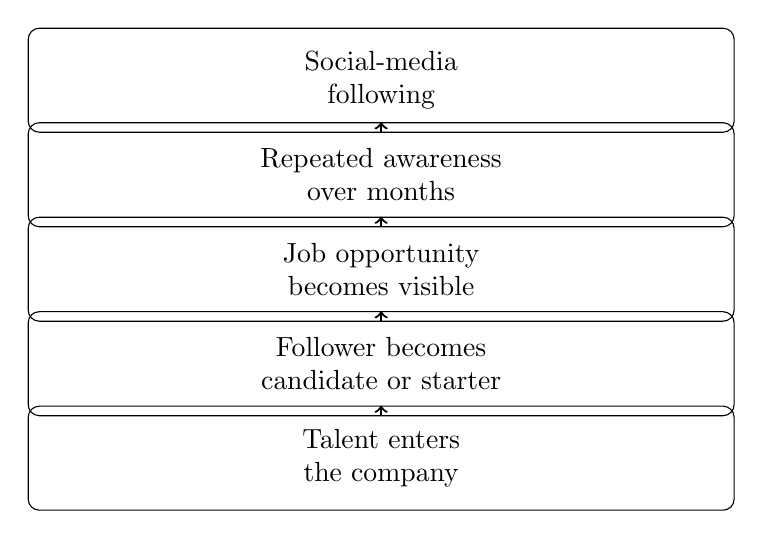
\begin{tikzpicture}[
  box/.style={draw, rounded corners, align=center, text width=0.72\linewidth, minimum height=0.52in},
  arrow/.style={->, thick}
]
\node[box] (a) at (0,0) {Social-media\\following};
\node[box] (b) at (0,-1.20) {Repeated awareness\\over months};
\node[box] (c) at (0,-2.40) {Job opportunity\\becomes visible};
\node[box] (d) at (0,-3.60) {Follower becomes\\candidate or starter};
\node[box] (e) at (0,-4.80) {Talent enters\\the company};

\draw[arrow] (a) -- (b);
\draw[arrow] (b) -- (c);
\draw[arrow] (c) -- (d);
\draw[arrow] (d) -- (e);
\end{tikzpicture}
\caption{Transcript-derived mechanism: social attention becomes recruiting visibility.}
\end{figure}

A useful way to keep the pieces separate is to distinguish stock from flow. The following is a stock:

\begin{equation}
A = F_T + F_I \approx 170{,}000.
\end{equation}

The hiring result is a flow event. It occurs only when that audience has repeated exposure and then encounters a concrete opportunity. As a cautious heuristic, not a measured law from the interview, we can write

\begin{equation}
\text{recruiting leverage}
\sim
\text{audience stock}
\times
\text{repeated exposure}
\times
\text{available opportunity}.
\end{equation}

The symbol \(\sim\) is intentional. This is not a calibrated formula. It is a way to keep the mechanism from collapsing into a slogan. The audience alone does not create a hire. The job alone may not reach the right person. The leverage appears when the right person has already been exposed to the company or founder and then sees a concrete opening.

\section{Source-Conscious Limits}

The evidence should be carried with its limits intact. The hiring meeting was small, with \(N=6\) or \(N=7\). The attribution range was spoken as an estimate. The role labeled ``RSM'' in the transcript is not expanded, so it should be treated simply as an internal company role or director-level participant unless another source clarifies it.

The strongest supported claim is therefore modest and practical:

\begin{equation}
\text{social media helped some new starters discover the company}.
\end{equation}

The transcript does not support a universal conversion rate, a platform comparison, or a claim that follower count alone explains hiring quality. What it does support is a concrete entrepreneurial mechanism: media visibility can widen the talent pool before the company formally asks for talent.

\section{Summary}

The excerpt begins with a question about leverage and resolves it through a recruiting example. Grant's stated audience, about \(145{,}000\) on TikTok and \(25{,}000\) on Instagram, is framed as meaningful but not massive. The evidence then shifts to a company-wide meeting with six or seven new starters, where roughly 30 to 40 percent reportedly traced their awareness back to following him.

The careful lesson is that social media is not only a marketing channel. In this segment, it functions as recruiting infrastructure. A person can follow for months, see an opening, and become part of the company. In entrepreneurial terms, that is leverage: prior attention converted into opportunity flow.